\documentclass[12pt]{article}
\usepackage{graphicx}
\usepackage{float}
\usepackage{tikz}
\usepackage{listings}
\usepackage{color}



\usetikzlibrary{arrows}
\usetikzlibrary{positioning}

\graphicspath{ {images/} }
\title{Project 1:\\Solving 2x2 RPM using Verbal and/or Visual Representations \\ Reflection}
\date{2015-09-6}

\definecolor{mygreen}{rgb}{0,0.6,0}
\definecolor{mygray}{rgb}{0.5,0.5,0.5}
\definecolor{mygreen}{rgb}{0.1,0.50,0.1}

\lstset{ %
  backgroundcolor=\color{white},   % choose the background color; you must add \usepackage{color} or \usepackage{xcolor}
  basicstyle=\footnotesize,        % the size of the fonts that are used for the code
  breakatwhitespace=false,         % sets if automatic breaks should only happen at whitespace
  breaklines=true,                 % sets automatic line breaking
  captionpos=b,                    % sets the caption-position to bottom
  commentstyle=\color{mygreen},    % comment style
  deletekeywords={...},            % if you want to delete keywords from the given language
  escapeinside={\%*}{*)},          % if you want to add LaTeX within your code
  extendedchars=true,              % lets you use non-ASCII characters; for 8-bits encodings only, does not work with UTF-8
  frame=single,	                   % adds a frame around the code
  keepspaces=true,                 % keeps spaces in text, useful for keeping indentation of code (possibly needs columns=flexible)
  keywordstyle=\color{blue},       % keyword style
  language=Octave,                 % the language of the code
  otherkeywords={*,...},            % if you want to add more keywords to the set
  numbers=none,                    % where to put the line-numbers; possible values are (none, left, right)
  numbersep=5pt,                   % how far the line-numbers are from the code
  numberstyle=\tiny\color{mygray}, % the style that is used for the line-numbers
  rulecolor=\color{black},         % if not set, the frame-color may be changed on line-breaks within not-black text (e.g. comments (green here))
  showspaces=false,                % show spaces everywhere adding particular underscores; it overrides 'showstringspaces'
  showstringspaces=false,          % underline spaces within strings only
  showtabs=false,                  % show tabs within strings adding particular underscores
  stepnumber=2,                    % the step between two line-numbers. If it's 1, each line will be numbered
  stringstyle=\color{mygreen},     % string literal style
  tabsize=2,	                   % sets default tabsize to 2 spaces
  title=\lstname                   % show the filename of files included with \lstinputlisting; also try caption instead of title
}

\begin{document}
	\pagenumbering{gobble}
	\maketitle
	\newpage
	\pagenumbering{arabic}
\section{Introduction}
	\paragraph{•}
	Raven's Progressive Matrices are visual analogy problems. They are one of the most commonly used intelligence tests. \cite{kaplan2009standardized} These visual analogies are pairs or series of images that contain some tangible pattern. Figure \ref{fig:b-06} is an example of such a problem from the CS7637: Knowledge-Based AI: Fall 2015 Class Documents:
	\begin{figure}[H]
	\centering
	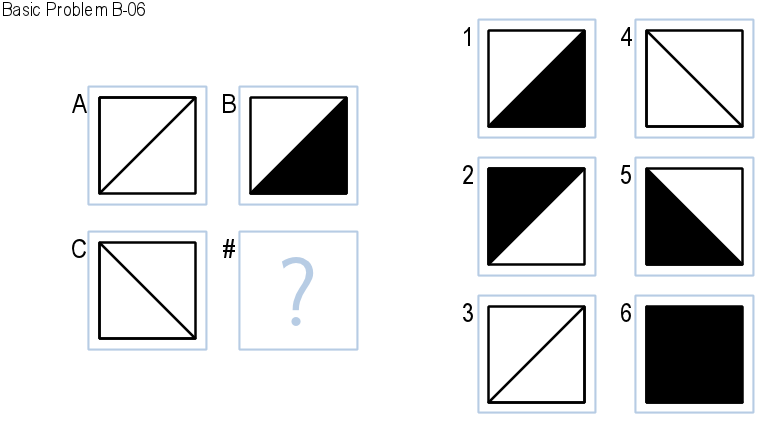
\includegraphics[width=0.5\textwidth]{Basic-Problem-B-06-2.png}
	 \caption{Basic Raven's Problem}
	 \label{fig:b-06}
	\end{figure}
	\paragraph{•}
	In this problem, the solution is 5. The pattern or relation from A to B is that one shape has been filled. The relation from A to C is that the image has been reflected over a vertical axis. Therefore, the solution must be a vertical reflection of B and have the same shapes as C except with one filled. 5 is the only candidate that meats this criteria and is therefore the solution. The goal of this assignment is to design a knowledge based artificial intelligence agent that can reason about Raven's Progressive Matrices and solve them. In particular, representing the knowledge of each image as a semantic network will enable the agent to solve basic problems by analyzing the changes between rows and columns of a matrix to find the solution.
	 \paragraph{•}
	 This problem is quite difficult; the agent needs to be able to capture all important meanings and relationships, without necessarily knowing which features are important or unimportant. Furthermore, the agent must consider or find short-cuts to avoid considering an entire exponential set of possible shape manipulations. The more shape manipulations the agent is aware of, the more it will need to consider to solve each problem. Since the manipulation domain is essentially unconstrained this is especially problematic.

\label{sec:reflection_q}
\section{Reflection Questions}
\subsection{How does your agent reason over the problems it receives? What is its overall problem-solving process? Did you take any risks in the design of your agent, and did those risks pay off?}
\paragraph{}
My AI agent uses a mix of frames and generate and test to reason about the RPM problems. A frame is a data structure used to store pieces of knowledge for stereotyped situations. \cite{minsky} Generate and test is exactly what it sounds like; the agent generates a solution and then tests it against candidate solutions to find an answer. The ultimate control flow for any problem the agent solves is as follows. 
\paragraph{}
First, create a frame for each object in each figure of the problem. Then, for Figure A and Figure B, attempt to produce a matching for each frame in A to another frame in B. Assign the closest matches first, and assume any unmatched frames are either added to B or deleted from A. The agent repeats this process for Figure A and Figure C.
\paragraph{}
Second, for each matching $(M_{AB})$, try to produce a series of transformations that would turn $A_1$ into $B_1$. The key here was to check possible transformations in order of likelihood. The agent has a list of transformations it can apply, and tries them in order until it finds something that turns $A_1$ into $B_1$. The agent then tries combinations of those transformations in lexicographic order. In this way it rapidly finds what it judges to be the ``simplest'' transformation by simple brute force. This was risky, as it is just slightly smarter brute force, but it paid off well enough since it was so fast. Here there is a chance for some more intelligence with means end analysis, which I will come back to later. Again, the agent repeats this process for Figure A and Figure C.
\paragraph{}
Thirdly, with the transformations, $T_{AB}$ and $T_{BC}$, in hand, apply the transformations across the diagonal. This means apply any transformations $T_{AB}$ using the mapping $(M_{AC})$, assuming that the matching must hold. This generates a possible solution $a_{AB}$. Repeating the process for $T_{AC}$ using the mapping $(M_{AB})$ generates another possible solution $c_{AB}$. If both generated solutions match, the agent is highly confident that the solution is correct, even before testing against the multiple choice answer figures. This is an interesting strength of this agent, it doesn't need to see candidate answers to find the answers. I would conjecture that human reasoning is likely similar for these especially basic problems. In any case, since there is no guessing disadvantage in project one, the agent simply chooses the first solution it finds that matches its generated solution, completing the generate and test cycle. 
\paragraph{}
While this was enough for the basic problems, this cycle could be repeated for different matching $M$ and different transformations $T$ that are valid, but considered more costly by the agent. If the agent finds a solution it is more confident about, it can record the transformations as more useful by decreasing their cost. After their cost is decreased it can change the lexicographic ordering of potential transformation combinations by sorting the list of transformations by cost. Thus the agent could learn about other potential solutions and when to apply them. I didn't get around to this, but look forward to trying when there are more problems in the problem set.
\paragraph{}
Another key risk that I took in programming this agent was to relax the definition of equivalence for hashes and equality of frames. I took position completely out of the hash and equality methods. My reasoning was that relational positions can change but a shape could still be equivalent to another. Consider the case where a shape is inside another, but the other shape is removed. In this case, we still want the shape to test as equal. This resulted in many gains but failed spectacularly when position was important. Ultimately, some way of reincorporating position will be necessary. 
\subsection{How does your agent actually select an answer to a given problem? What metrics, if any, does it use to evaluate potential answers? Does it select only the exact correct answer, or does it rate answers on a more continuous scale?}
\paragraph{}
While it is not immediately obvious, this agent does indeed use a metric to evaluate potential answers. The metric is implicit in the cost of various transformations. The agent will answer with the first valid transformation sequence it finds. It generates these by going over an ordering of transformation combinations sorted by cost. Thus, the total cost of the transformations used is the ultimate metric that the agent uses to select an answer. The unsatisfying part of this is that it still only selects one exact correct answer. The benefit is that the agent has room to learn by modifying the ordering of the transformation combinations. It could even store this order between subsequent runs of the program on different problem sets, learning more and more about which transformations are more common or less common. 

\subsection{What mistakes does your agent make? Why does it make these mistakes? Could these mistakes be resolved within your agent’s current approach, or are they fundamental problems with the way your agent approaches these problems?}
\paragraph{}
One major issue the agent has is distinguishing between rotations of objects that are not symmetrical. For example, the right triangles used in Figure \ref{fig:b-06}. Since the agent does not use positional data when comparing for equality, the verbal descriptions were insufficient to determine the orientation of these figures, thus mirroring them properly was impossible. In this particular case, the agent would randomly reason that it could either rotate the triangles left by 90 degrees or right by 90 degrees. In one case, this would map to the correct solution, 5, in the other, it would generate a solution like 5 but with the fills flipped. The agent has no way to properly understand this reflection. This could potentially be resolved by bringing positional information back into the agents reasoning, though I would hesitate to put it back into shape equality. Ideally, a frame that represented the figure as a whole and could be compared, mirrored, or rotated would probably be the way to go. Luckily, an image representation of the figure is a good way to accomplish that, and I plan to focus my efforts there. 

\subsection{What improvements could you make to your agent given unlimited time and resources? How would you implement those improvements? Would those improvements improve your agent’s accuracy, efficiency, generality, or something else?}
\paragraph{}
I've already mentioned some of these above, but I will list them here again as well.
\paragraph{}
First, the agent could use means-ends analysis in lieu of the brute force approach to searching the combinatorial space of transformations. Essentially, this would involve looking for any transformation that could get a shape closer to the target shape, selecting that transformation, and then continuing. This would be pretty easy to implement as the logic for similarity between shapes is already present in the agent (it uses that logic to figure out how shapes correspond across figures). This would increase the agent's efficiency. 

\paragraph{}
Extending that idea a little bit, the agent could even skip having a starting list of transformations altogether. This would work by creating the list on the fly. The items on this list could be represented by the difference between two frames once frames are matched between figures. For example, if the top left triangles of A and B were 1 and 2 respectively, the agent would learn that there is a transformation to try that involves doing nothing (since 1 and 2 are the same). This would increase the agent's generality. While a lofty idea it does present a benefit, complex transformations like $T:(rotate, fill)$ could become one step transformations and weighted in a flat list.

\paragraph{}
I mentioned learning by modifying the costs of the list of transformations before. This type of learning would mostly impact the efficiency of the agent, but would also likely increase it's accuracy as it learned what types of transformations are more 'correct' than others.

\paragraph{}
One thing worth noting is that this agent does not leverage the visual representations of the problems at all. The visual representations present some key advantages for simply detecting what appear to be common transformations like reflection over the horizontal or vertical axis. Adding in some logic before the agent tries to decipher the problem through verbal reasoning could 'shortcut' the problem quite well. This would possibly improving accuracy generality, and efficiency all at once. Having a strong verbal reasoning system is still a good fallback however. 

\subsection{How well does your agent perform across multiple metrics? Accuracy is important, but what about efficiency? What about generality? Are there other metrics or scenarios under which you think your agent’s performance would improve or suffer?}
\paragraph{}
Without anything to compare against, I would have to say the agent is quite speedy. It is able to correctly complete all 12 problems in the B basic problem set in ~.4 seconds in the worst case over 10 runs. This was a surprising result to me, I expected to spend a lot of time optimizing the approach with some of the ideas above but found that a straightforward approach was good enough. Accuracy wise, the agent gets 11/12 of the basic problems correct. I am worried however that it is over fitted to the problem space. Without any other problem sets with verbal descriptions though it is impossible to test. When it comes to generality, the agent is a mixed bag. While I have no hard numbers since the Challenge problems do not have verbal descriptions, I doubt my agent could solve many of them anyway. Looking carefully over the problems and their solutions, I estimate that given verbal descriptions my agent might be able to solve 3 or 4 of the problems.

\subsection{Which reasoning method did you choose? Are you relying on verbal representations or visual? If you’re using visual input, is your agent processing it into verbal representations for subsequent reasoning, or is it reasoning over the images themselves?}
\paragraph{}
My agent is relying on entirely verbal representations. I hope to leverage raw images for reasoning, then fallback to processing those images into verbal descriptions to solve with this agent before giving up for future iterations of the project. 
\subsection{Finally, what does the design and performance of your agent tell us about human cognition? Does your agent solve these problems like a human does? How is it similar, and how is it different? Has your agent’s performance given you any insights into the way people solve these problems?}
\paragraph{}
The agent has some interesting characteristics that give us some clues about human cognition. The first, which I mentioned earlier, is that using generate and test the agent is able to come up with potential solutions even when solutions are not provided. Human cognition shows similar ability. One difference is that my agent can only reason about transitions it knows about. It can compose those transitions into sequences, but at great combinatorial cost. Some of the enhancements I propose would hopefully fix that problem.
\paragraph{}
Another key difference is the speed. No human being could process all 12 problems as quickly as the agent can, despite using a comparatively slow language like python without any multiprocessing. This is one of the likely goals of artificial intelligence, to process intelligence problems faster than a human being.
\paragraph{}
While developing the agent, it surprised me with several valid answers to problems that I hadn't initially considered. For example, problem B-04 with filled pac-man shapes mirrored over different axises. The agent initially decided that rotating the pacmans clockwise or counterclockwise was the correct transformation. This transformation is logically valid, but ends up with the unintuitive result of a pacman in the same orientation as it started. I think humans would reject this solution primarily because the a figure in the question is being reused in the answer and the answer doesn't complete a larger pattern. Humans tend to seek out patterns, and 'completing the box' as mentioned in the lecture is a an easy visual pattern to see. 

\section{Extra Implementation Details}
\paragraph{}
This section contains extra verbose implementation details. I moved them here to streamline the paper a little bit since it was getting long and these details aren't strictly necessary. 
\paragraph{Frames Upgraded}
I took frames one step further and made a full object class definition for shape frames in Python3. This frame class had several useful features. The first, and most important was that I made sure that it could be tested for equality against other frames quickly. To that end, I wrote two methods, \_\_eq\_\_ and
\_\_hash\_\_ , which are common in python. These methods allow frames to be used in sets, and for those sets, once frozen, to be further nested or compared against other sets very quickly. I also added a diff method. It could compare two different shape frames and find all the differences between them. It would then weight those differences. For example, a size change from small to huge is more weight than from very large to huge. This was especially useful when trying to match shapes across figures. It was always the case that the most similar shape between figures had somehow been transformed. Once the agent identified that transformation, it could apply it 'across the diagonal'.
\paragraph{Verbs}
My agent utilized a set of atomic transitions I called verbs and used those to compose transitions between frames. For each verb, I wrote a method that would transform one frame into another as the verb implied. For example, I created a 'unchanged' verb. This verb simply returned what was passed to it. A more complex example, the verb mirror\_ left\_ right verb could mirror (some) shapes over the Y axis using a little geometry. Each of these verbs were assigned a cost. To compose more complex transitions, combinations of verbs could be chained together. The result frame could be tested for inequality against another frame, establishing a list of shape differences or deltas between figures.

	\newpage
	
	\bibliographystyle{apalike}
	\bibliography{Project1}
\end{document}